\documentclass[10pt,twocolumn,letterpaper]{article}
\usepackage{comment}

\usepackage[utf8]{inputenc}
\usepackage{caption}
\usepackage{tabularx}
\captionsetup[table]{skip=20pt}
\usepackage{cvpr}
\usepackage{mathptmx}
\usepackage{graphicx}
\usepackage{amsmath}
\usepackage{siunitx}
\usepackage{physics}
\usepackage{amssymb}
\usepackage{tikz}
\usepackage{pgfplots}
\usepackage{subcaption}
\usepackage{bm,color}
\usetikzlibrary{arrows.meta}
\usetikzlibrary{shapes, arrows}
\usepackage{graphics}
\usepackage{pifont}
\pgfplotsset{compat=newest}
\usepackage{blindtext}

\usepackage[pagebackref=true,breaklinks=true,letterpaper=true,colorlinks,bookmarks=false]{hyperref}


\newcommand{\cmark}{\ding{51}}
\newcommand{\xmark}{\ding{55}}

% Init and set plot shapes
\newlength\figH
\newlength\figW
\setlength{\figH}{4cm}
\setlength{\figW}{8cm}

% Input tud colors
\definecolor{tud0d}{cmyk/RGB/HTML}{0,0,0,.8/83,83,83/535353}
\definecolor{tud0c}{cmyk/RGB/HTML}{0,0,0,.6/137,137,137/898989}
\definecolor{tud0b}{cmyk/RGB/HTML}{0,0,0,.4/181,181,181/B5B5B5}
\definecolor{tud0a}{cmyk/RGB/HTML}{0,0,0,.2/220,220,220/DCDCDC}
\definecolor{tud1a}{cmyk/RGB/HTML}{.7,.4,0,0/93,133,195/5D85C3}
\definecolor{tud2a}{cmyk/RGB/HTML}{0.8,.2,0,0/0,156,218/009CDA}
\definecolor{tud3a}{cmyk/RGB/HTML}{0.7,0,.5,0/80,182,149/50B695}
\definecolor{tud4a}{cmyk/RGB/HTML}{.4,0,.8,0/175,204,80/AFCC50}
\definecolor{tud5a}{cmyk/RGB/HTML}{.2,0,.8,0/221,223,72/DDDF48}
\definecolor{tud6a}{cmyk/RGB/HTML}{0,.1,.7,0/255,224,92/FFE05C}
\definecolor{tud7a}{cmyk/RGB/HTML}{0,.3,.8,0/248,186,60/F8BA3C}
\definecolor{tud8a}{cmyk/RGB/HTML}{0,.6,.8,0 /238,122,52/EE7A34}
\definecolor{tud9a}{cmyk/RGB/HTML}{0,.8,.7,0/233,80,62/E9503E}
\definecolor{tud10a}{cmyk/RGB/HTML}{.2,.9,0,0/201,48,142/C9308E}
\definecolor{tud11a}{cmyk/RGB/HTML}{.6,.8,0,0/128,69,151/804597}
\definecolor{tud1b}{cmyk/RGB/HTML}{1,.6,0,0/0,90,169/005AA9}
\definecolor{tud2b}{cmyk/RGB/HTML}{1,.3,0,0/0,131,204/0083CC}
\definecolor{tud3b}{cmyk/RGB/HTML}{1,0,.6,0/0,157,129/009D81}
\definecolor{tud4b}{cmyk/RGB/HTML}{.5,0,1,0/153,192,0/99C000}
\definecolor{tud5b}{cmyk/RGB/HTML}{.3,0,1,0/201,212,0/C9D400}
\definecolor{tud6b}{cmyk/RGB/HTML}{0,.2,1,0/253,202,0/FDCA00}
\definecolor{tud7b}{cmyk/RGB/HTML}{0,.4,1,0/245,163,0/F5A300}
\definecolor{tud8b}{cmyk/RGB/HTML}{0,.7,1,0/236,101,0/EC6500}
\definecolor{tud9b}{cmyk/RGB/HTML}{0,1,.9,0/230,0,26/E6001A}
\definecolor{tud10b}{cmyk/RGB/HTML}{.4,1,0,0/166,0,132/A60084}
\definecolor{tud11b}{cmyk/RGB/HTML}{.7,1,0,0/114,16,133/721085}
\definecolor{tud1c}{cmyk/RGB/HTML}{1,.7,.2,0/0,78,138/004E8A}
\definecolor{tud2c}{cmyk/RGB/HTML}{1,.5,.2,0/0,104,157/00689D}
\definecolor{tud3c}{cmyk/RGB/HTML}{1,.2,.6,0/0,136,119/008877}
\definecolor{tud4c}{cmyk/RGB/HTML}{.6,.1,1,0/127,171,22/7FAB16}
\definecolor{tud5c}{cmyk/RGB/HTML}{.4,.1,1,0/177,189,0/B1BD00}
\definecolor{tud6c}{cmyk/RGB/HTML}{.2,.3,1,0/215,172,0/D7AC00}
\definecolor{tud7c}{cmyk/RGB/HTML}{.2,.5,1,0/210,135,0/D28700}
\definecolor{tud8c}{cmyk/RGB/HTML}{.2,.8,1,0/204,76,3/CC4C03}
\definecolor{tud9c}{cmyk/RGB/HTML}{.3,1,.9,0/185,15,34/B90F22}
\definecolor{tud10c}{cmyk/RGB/HTML}{.5,1,.3,0/149,17,105/951169}
\definecolor{tud11c}{cmyk/RGB/HTML}{.8,1,.2,0/97,28,115/611C73}
\definecolor{tud1d}{cmyk/RGB/HTML}{1,.9,.3,0/36,53,114/243572}
\definecolor{tud2d}{cmyk/RGB/HTML}{1,.7,.4,0/0,78,115/004E73}
\definecolor{tud3d}{cmyk/RGB/HTML}{1,.4,.7,0/0,113,94/00715E}
\definecolor{tud4d}{cmyk/RGB/HTML}{.7,.3,1,0/106,139,55/6A8B22}
\definecolor{tud5d}{cmyk/RGB/HTML}{.5,.2,1,0/153,166,4/99A604}
\definecolor{tud6d}{cmyk/RGB/HTML}{.4,.4,1,0/174,142,0/AE8E00}
\definecolor{tud7d}{cmyk/RGB/HTML}{.3,.6,1,0/190,111,0/BE6F00}
\definecolor{tud8d}{cmyk/RGB/HTML}{.4,.8,1,0/169,73,19/A94913}
\definecolor{tud9d}{cmyk/RGB/HTML}{.5,1,.9,0/156,28,38/961C26}
\definecolor{tud10d}{cmyk/RGB/HTML}{.7,1,.5,0/115,32,84/732054}
\definecolor{tud11d}{cmyk/RGB/HTML}{.9,1,.3,0/76,34,106/4C226A}

% Math styles
\newcommand{\Vector}[1]{\boldsymbol{#1}}
\newcommand{\Matrix}[1]{\boldsymbol{\MakeUppercase{#1}}}
\newcommand{\Tensor}[1]{\boldsymbol{\mathrm{\MakeUppercase{#1}}}}
\newcommand{\Set}[1]{\mathbb{#1}}
\newcommand{\Mean}[1]{\mathbb{E}\left[#1\right]}
\newcommand{\Var}[1]{\mathrm{Var}\left[#1\right]}
\newcommand{\Cov}[1]{\mathrm{Cov}\left[#1\right]}
\newcommand{\Gaussian}[1]{\mathcal{N}\left(#1\right)}

\cvprfinalcopy

\def\httilde{\mbox{\tt\raisebox{-.5ex}{\symbol{126}}}}

\setcounter{page}{1}
\begin{document}

\title{DeepFovea++: Reconstruction and Super-Resolution for Natural Foveated Rendered Videos}

\author{
    Christoph Reich\\
    TU Darmstadt\\
    {\tt\small christoph.reich@stud.tu-darmstadt.de}
    
    \and
    Marius Memmel\\
    TU Darmstadt\\
    {\tt\small marius.memmel@stud.tu-darmstadt.de}
    
    \and
    Jonas Henry Grebe\\
    TU Darmstadt\\
    {\tt\small jonas.grebe@stud.tu-darmstadt.de}
}


\twocolumn[{%
\renewcommand\twocolumn[1][]{#1}%
\maketitle
\begin{center}
    \centering
    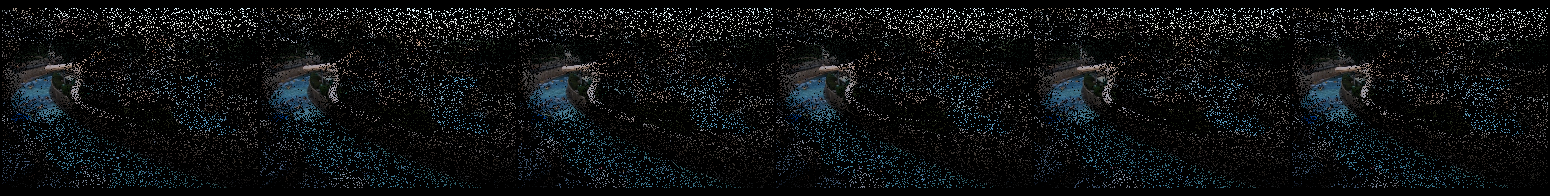
\includegraphics[width=\textwidth]{figures/input.png}\\\vspace{-0.1cm}
    \includegraphics[width=\textwidth]{figures/prediction.png}\\\vspace{-0.1cm}
    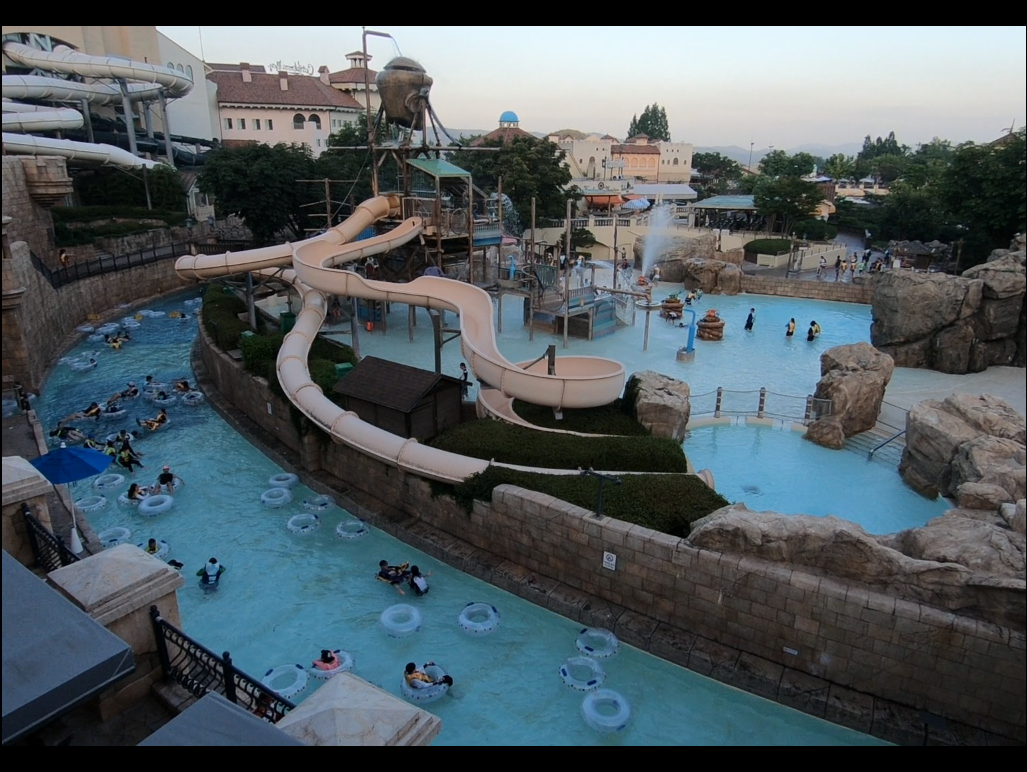
\includegraphics[width=\textwidth]{figures/label.png}\\
    \captionof{figure}{Results of our proposed DeepFovea++ technique. The fovea sampled input sequences of low resolution (192 X 256) image frames can be seen on the top. The reconstructed super-resolution (768 X 1024) prediction sequence is shown in the middle, and the corresponding label at the bottom.}
    \label{fig:firstresults}
\end{center}%
}]

\begin{abstract}
Image super-resolution is a well-known problem in the computer vision community. Recent papers extended the problem of super-resolution to videos and showed amazing results. On the other hand deep learning based fovea sampled image reconstruction has drawn some popularity since the DeepFovea publication of Facebook AI. DeepFovea showed outstanding results, however, the proposed reconstruction network was only able to reconstruct relatively low-resolution images of $128\times128$ pixels. We revisit the proposed DeepFovea architecture to perform fovea sampled video reconstruction and super-resolution ($192 \times 256$ $\to$ $768 \times 1024$) at once. Our proposed architecture, DeepFovea++, first reconstructs a given video sequence by a recurrent U-Net architecture, and afterward, the desired super-resolution is learned by deformable convolutions. We tested our DeepFovea++ architecture on the challenging REDS dataset. The code is available at \url{https://github.com/ChristophReich1996/DeepFoveaPP_for_Video_Reconstruction_and_Super_Resolution}.
\end{abstract}

\section{Introduction} % Jonas

\section{Previous Work} % Marius

\section{DeepFovea++ Architecture} % Christoph
The DeepFovea++ reconstruction model is mainly based on two parts. First, a recurrent residual U-Net \cite{unet, deepfovea}, and second, two super-resolution blocks based on deformable convolutions. We train both, the U-Net, and the super-resolution blocks, in an end-to-end setting. The whole reconstruction architecture consists of about 2.3 Mio parameters. We used a relatively small reconstruction model to be able to fit the whole DeepForvea++ framework, consisting of the reconstruction model, a 3d discriminator, and a 3D FFT-discriminator, into GPU memory.

\subsection{Reconstruction model}

\subsection{Discriminator}

\subsection{FFT-Discriminator}

\subsection{Lossfunction}

\subsubsection{Supervised loss}

\subsubsection{Adversarial loss}

\subsubsection{Flow loss}

\section{Experiments} % Christoph

\subsection{REDS Dataset} % Jonas

\subsection{Implementation Details} % Christoph
We implemented the whole DeepFovea++ framework in PyTorch 1.4.0 \cite{pytorch}. Our implementation is based on multiple existing implementations. First, we build our framework on top of the deformable convolution v2 \cite{deformableconv} implementation included in the mmdetection toolbox \cite{mmdetection}. Second, we used the correlation package \cite{flownet2} of Nvidia for implementing the optical flow loss. Furthermore, to estimate the optical flow for the corresponding optical flow loss, we utilized a pre-trained PWC-Net \cite{pwcnet} by Nvidia research. Finally, our main supervised loss function is based on the adaptive robust loss function implementation by Jonathan T. Barron \cite{adaptiveroubustloss}.\\
For optimizing all networks we utilized the Adam optimizer \cite{adam}. For the reconstruction model, we set the learning rate to $3\times 10^{-4}$. The first and second-order running average factors were set 0.1 and 0.95, respectively. In both the 3d discriminator and the 3d FFT-discriminator we set the learning rate to $10^{-4}$. The first and second-order running average factors were set to the same value as for the reconstruction model.\\

TODO: Fovea mask!\\

TODO: Preprcessing\\

We were able to fit one sequence consisting of six rgb frames on one Tesla V100 (16GB). We trained our whole framework for 15 epochs on two GPUs. This results in a batch size of two. This training process took us about two days.

\subsection{Results} % Christoph
For analyzing our framework results we calculated multiple metrics. First, we compute the common $\operatorname{L1}$ metric and the Mean-Squared-Error (MSE, $\operatorname{L2}$). In case for a reconstructed image $\Tensor{I}_{\text{pred}}\in\Set{R}^{c, h, w}$ and the corresponding label $\Tensor{I}_{\text{label}}\in\Set{R}^{c, h, w}$, the $\operatorname{L1}$ and $\operatorname{L2}$ loss is defined as

\begin{align}
    \operatorname{L1} &= \frac{1}{n\times c\times w}\norm{\Tensor{I}_{\text{pred}} - \Tensor{I}_{\text{label}}}_{1}\\
    \operatorname{L2} &= \frac{1}{n\times c\times w}\norm{\Tensor{I}_{\text{pred}} - \Tensor{I}_{\text{label}}}_{2}.
\end{align}

Additionally we compute the Peak-Signal-ToNoise ($\operatorname{PSNR}$) and the, and Structural-Similarity-Image-Metric ($\operatorname{SSIM}$) \cite{ssmi} to evaluate quality of prediction, which are defined as

\begin{align}
    \operatorname{PSNR}&=10 \log_{10},\left(\frac{\max\{\Tensor{I}_{\text{pred}}\}^2}{\operatorname{L2}\left(\Tensor{I}_{\text{pred}}, \Tensor{I}_{\text{label}}\right)} \right)\\
    \operatorname{SSIM}&=\frac{4\Mean{\Tensor{I}_{\text{pred}}}\Mean{\Tensor{I}_{\text{label}}}\Cov{\Tensor{I}_{\text{pred}}, \Tensor{I}_{\text{label}}}}{\left(\Mean{\Tensor{I}_{\text{pred}}}^2 + \Mean{\Tensor{I}_{\text{label}}}^2\right)\left(\Var{\Tensor{I}_{\text{pred}}} + \Var{\Tensor{I}_{\text{label}}}\right)}.
\end{align}

We tested our DeepFovea++ framework with two settings. In the first setting, we reset the recurrent state of the reconstruction model after each video sequence. In the second setting, we preserve the recurrent state over the whole training and validation process. Our tests lead to the following results.\\

TODO: Insert results\\

\section{Conclusion} % All

{\small
    \bibliographystyle{ieee}
    \bibliography{egbib}
}

\section{Appendix}

\begin{figure}[h!]
    \centering
    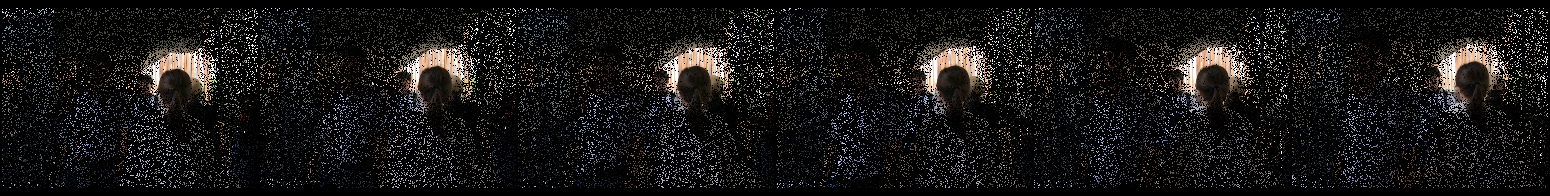
\includegraphics[width=\columnwidth]{figures/no_rest/input_83_2020-05-06 09_56_21.383738.png}\\\vspace{-0.1cm}
    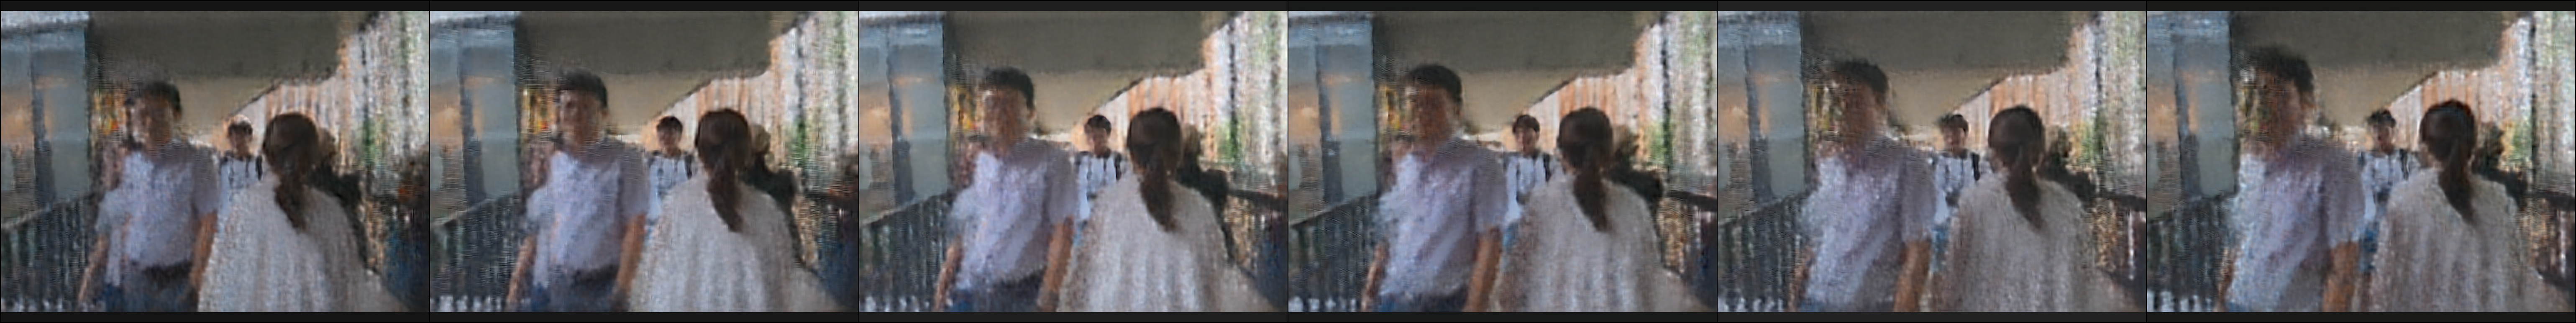
\includegraphics[width=\columnwidth]{figures/no_rest/prediction_83_2020-05-06 09_56_17.234900.png}\\\vspace{-0.1cm}
    \includegraphics[width=\columnwidth]{figures/no_rest/label_83_2020-05-06 09_56_19.447333.png}\\
    \caption{Results of the first DeepFovea++ setting. The fovea sampled input sequences (192 X 256) on the top. The reconstructed super-resolution (768 X 1024) prediction sequence in the middle, and the corresponding label at the bottom.}
    \label{fig:norestresults1}
\end{figure}

\begin{figure}[h!]
    \centering
    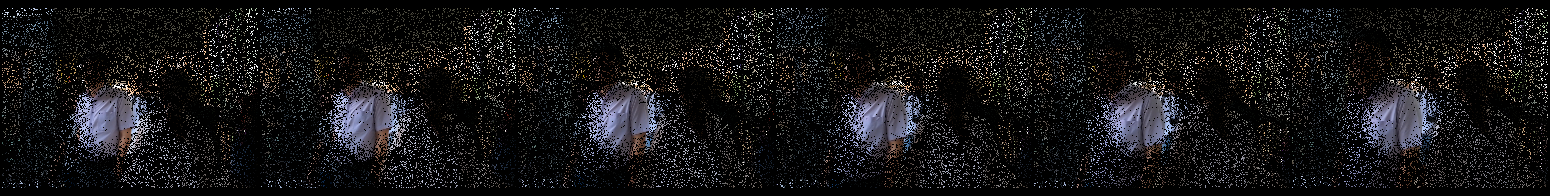
\includegraphics[width=\columnwidth]{figures/rest/input_83_2020-05-04 11_16_57.840082.png}\\\vspace{-0.1cm}
    \includegraphics[width=\columnwidth]{figures/rest/prediction_83_2020-05-04 11_16_53.597074.png}\\\vspace{-0.1cm}
    \includegraphics[width=\columnwidth]{figures/rest/label_83_2020-05-04 11_16_55.895397.png}\\
    \caption{Results of the second DeepFovea++ setting. The fovea sampled input sequences (192 X 256) on the top. The reconstructed super-resolution (768 X 1024) prediction sequence in the middle, and the corresponding label at the bottom.}
    \label{fig:restresults1}
\end{figure}

\begin{figure}[h!]
    \centering
    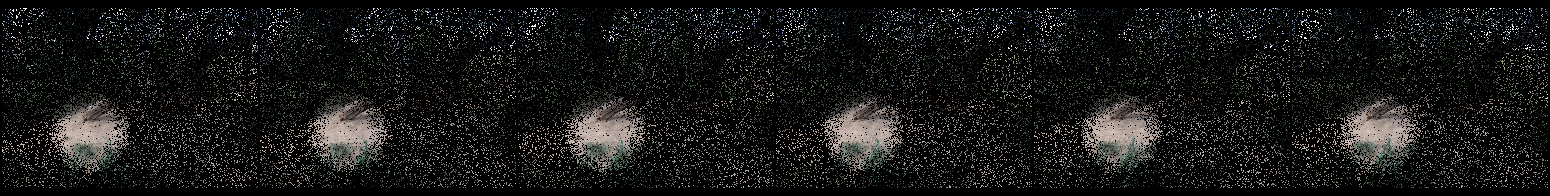
\includegraphics[width=\columnwidth]{figures/no_rest/input_432_2020-05-06 09_58_44.696719.png}\\\vspace{-0.1cm}
    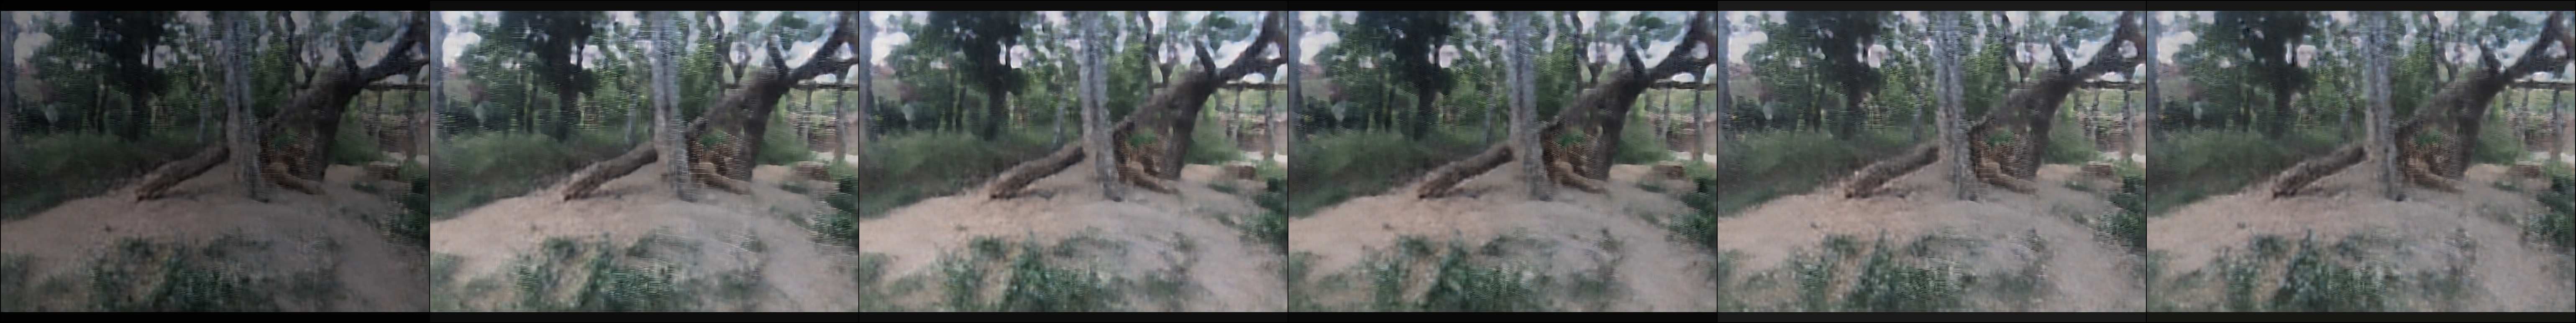
\includegraphics[width=\columnwidth]{figures/no_rest/prediction_432_2020-05-06 09_58_40.811600.png}\\\vspace{-0.1cm}
    \includegraphics[width=\columnwidth]{figures/no_rest/label_432_2020-05-06 09_58_43.122398.png}\\
    \caption{Results of the first DeepFovea++ setting. The fovea sampled input sequences (192 X 256) on the top. The reconstructed super-resolution (768 X 1024) prediction sequence in the middle, and the corresponding label at the bottom.}
    \label{fig:norestresults2}
\end{figure}

\begin{figure}[h!]
    \centering
    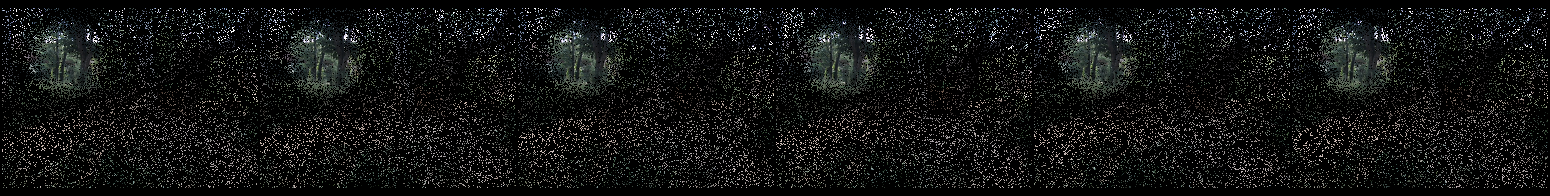
\includegraphics[width=\columnwidth]{figures/rest/input_432_2020-05-04 11_19_22.304534.png}\\\vspace{-0.1cm}
    \includegraphics[width=\columnwidth]{figures/rest/prediction_432_2020-05-04 11_19_18.114088.png}\\\vspace{-0.1cm}
    \includegraphics[width=\columnwidth]{figures/rest/label_432_2020-05-04 11_19_20.713044.png}\\
    \caption{Results of the second DeepFovea++ setting. The fovea sampled input sequences (192 X 256) on the top. The reconstructed super-resolution (768 X 1024) prediction sequence in the middle, and the corresponding label at the bottom.}
    \label{fig:restresults2}
\end{figure}

\begin{figure}[h!]
    \centering
    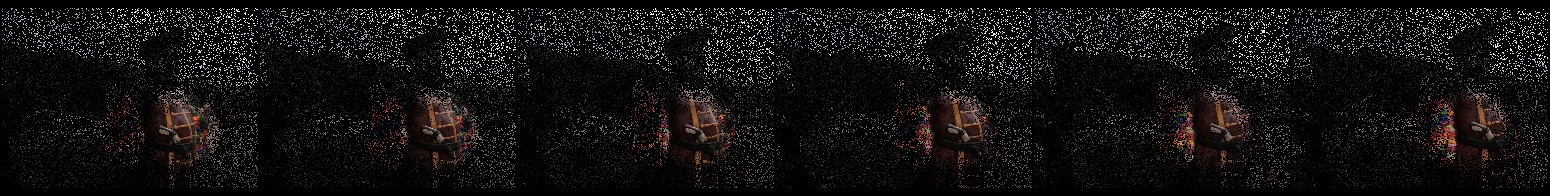
\includegraphics[width=\columnwidth]{figures/no_rest/input_150_2020-05-06 09_56_53.103463.png}\\\vspace{-0.1cm}
    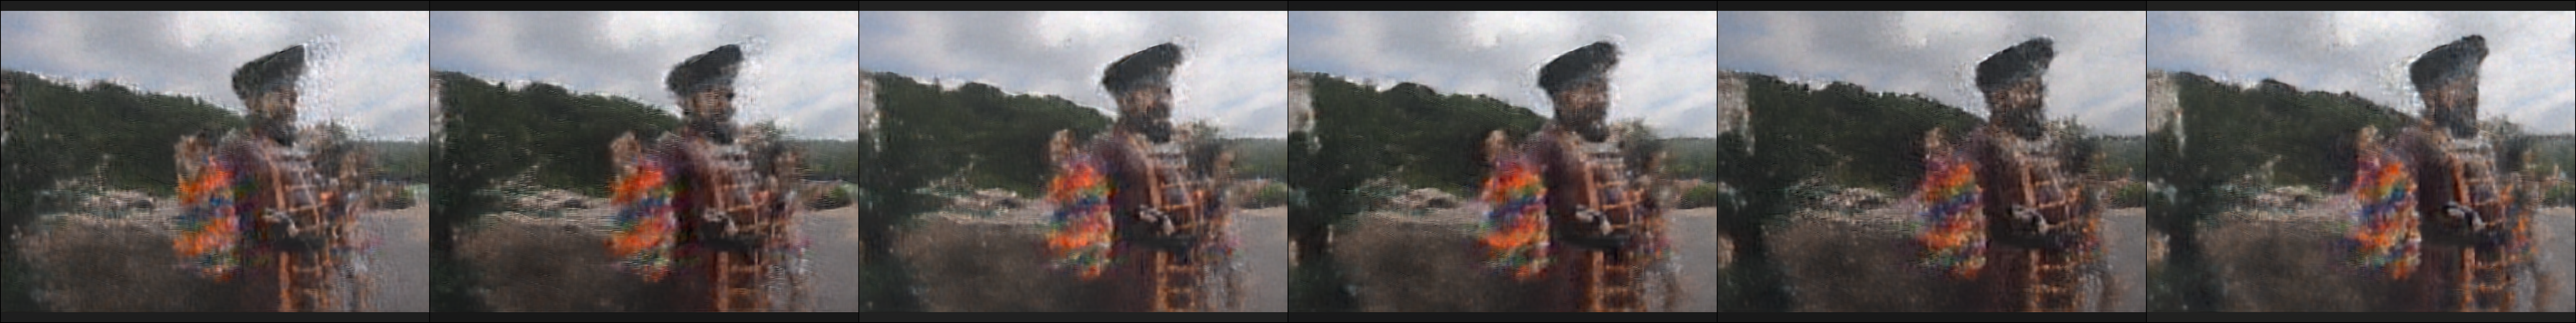
\includegraphics[width=\columnwidth]{figures/no_rest/prediction_150_2020-05-06 09_56_48.941222.png}\\\vspace{-0.1cm}
    \includegraphics[width=\columnwidth]{figures/no_rest/label_150_2020-05-06 09_56_51.153540.png}\\
    \caption{Results of the first DeepFovea++ setting. The fovea sampled input sequences (192 X 256) on the top. The reconstructed super-resolution (768 X 1024) prediction sequence in the middle, and the corresponding label at the bottom.}
    \label{fig:norestresults3}
\end{figure}

\begin{figure}[h!]
    \centering
    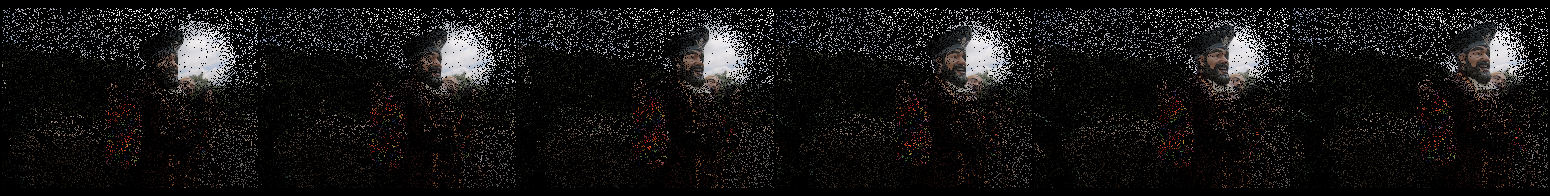
\includegraphics[width=\columnwidth]{figures/rest/input_150_2020-05-04 11_17_29.891315.png}\\\vspace{-0.1cm}
    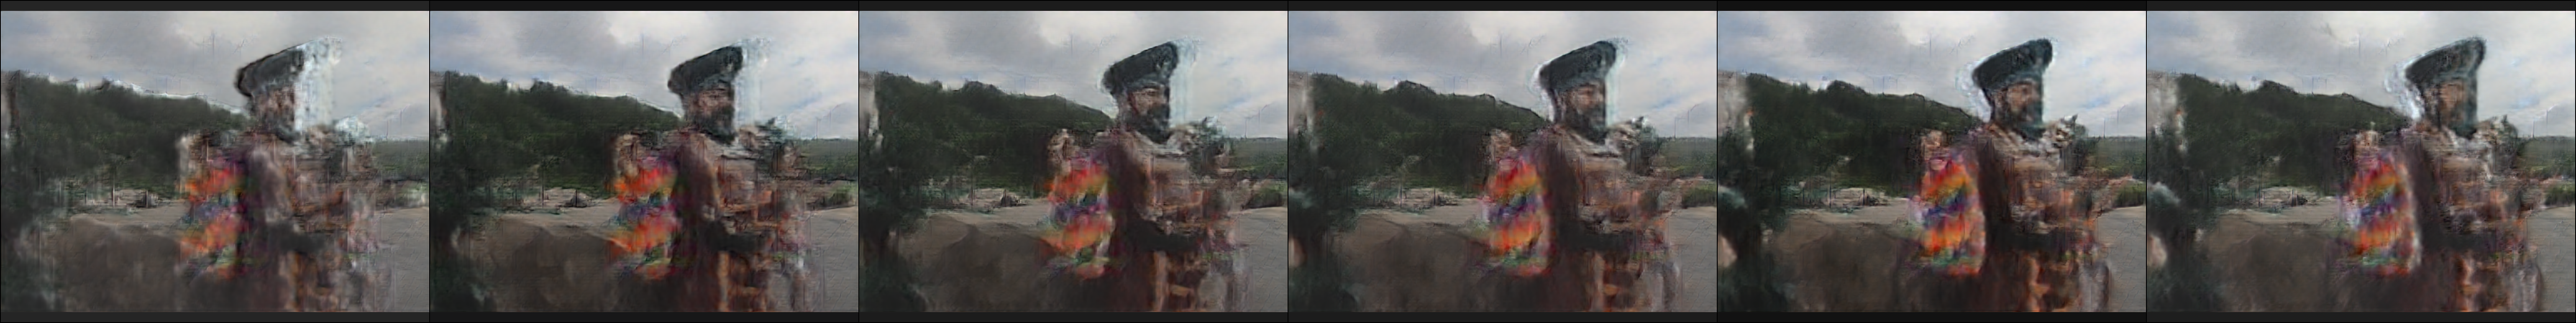
\includegraphics[width=\columnwidth]{figures/rest/prediction_150_2020-05-04 11_17_25.749898.png}\\\vspace{-0.1cm}
    \includegraphics[width=\columnwidth]{figures/rest/label_150_2020-05-04 11_17_27.920524.png}\\
    \caption{Results of the second DeepFovea++ setting. The fovea sampled input sequences (192 X 256) on the top. The reconstructed super-resolution (768 X 1024) prediction sequence in the middle, and the corresponding label at the bottom.}
    \label{fig:restresults3}
\end{figure}

\end{document}